% ------------------------------------------------------------------------------
% TYPO3 CMS 6.2 LTS - What's New - Chapter "Install Tool" (English Version)
%
% @author	Michael Schams <schams.net>
% @license	Creative Commons BY-NC-SA 3.0
% @link		http://typo3.org/download/release-notes/whats-new/
% @language	English
% ------------------------------------------------------------------------------
% Chapter: Install Tool
% ------------------------------------------------------------------------------
\section{Instalator}
\begin{frame}[fragile]
	\frametitle{Instalator (Install Tool)}

	\begin{center}\huge{Rozdział 1:}\end{center}
	\begin{center}\huge{\color{typo3darkgrey}\textbf{Instalator}}\end{center}

\end{frame}

% ------------------------------------------------------------------------------
% Installation
% ------------------------------------------------------------------------------

\begin{frame}[fragile]
	\frametitle{Instalator (Install Tool)}
	\framesubtitle{Instalacja}

	\begin{itemize}
		\item Tylko \underline{jedna} paczka wymagana jest do instalacji:\newline
				\texttt{typo3\_src-6.2.x.tar.gz} (rozmiar pliku: ok 20MB)
		\item Paczki "Dummy" oraz "Blank" stały się niepotrzebne
		\item Przebieg instalacji:
			\begin{itemize}
				\item Wypakuj archiwum z kodem źródłowym
				\item Stwórz odpowiednie dowiązania symboliczne
				\item Otwórz stronę w przeglądarce
				\item Podążaj za kolejnymi krokami instalatora TYPO3
			\end{itemize}

	\end{itemize}

\end{frame}

% ------------------------------------------------------------------------------
% Installation
% ------------------------------------------------------------------------------

\begin{frame}[fragile]

	\frametitle{Instalator (Install Tool)}
	\framesubtitle{Instalacja}

	\begin{itemize}
		\item Instalator sprawdza czy wszystkie potrzebne pliki i foldery są na miejscu
		\item Automatycznie tworzy pliki konfiguracyjne
		\item Poniższe dowiązania symboliczne \underline{muszą} istnieć:

		\begin{itemize}
			\item \texttt{typo3\_src}	\tabto{2cm} (wskazuje na folder ze źródłami TYPO3)
			\item \texttt{typo3}		\tabto{2cm} (wskazuje na folder: \texttt{typo3\_src/typo3})
			\item \texttt{index.php}	\tabto{2cm} (wskazuje na plik: \texttt{typo3\_src/index.php})
		\end{itemize}

		\item Nie potrzeba żadnych dodatkowych plików/folderów do instalacji TYPO3!
		\item Folder \texttt{t3lib} został usunięty
		\item Więcej informacji - zobacz: Poradnik instalacji i aktualizacji TYPO3\newline
			\url{http://docs.typo3.org/typo3cms/InstallationGuide}

	\end{itemize}

\end{frame}

% ------------------------------------------------------------------------------
% Re-Development
% ------------------------------------------------------------------------------

\begin{frame}[fragile]
	\frametitle{Instalator (Install Tool)}
	\framesubtitle{Zmiany w instalatorze}

	\begin{columns}[T]

		\begin{column}{.5\textwidth}
			\begin{itemize}
				\item Został przepisany od nowa\newline z użyciem szablonów Fluid
				\item \underline{Pierwszy} krok testuje system i raportuje problemy
				\item Znalezione problemy mogą zostać naprawione\newline (i przetestowane ponownie) lub zignorowane
				\item Nieprawidłowa instalacja jądra systemu (np. brak dowiązań symbolicznych) jest również raportowana jako problem
			\end{itemize}
		\end{column}

		\begin{column}{.5\textwidth}
			\begin{figure}\vspace*{-0.4cm}
				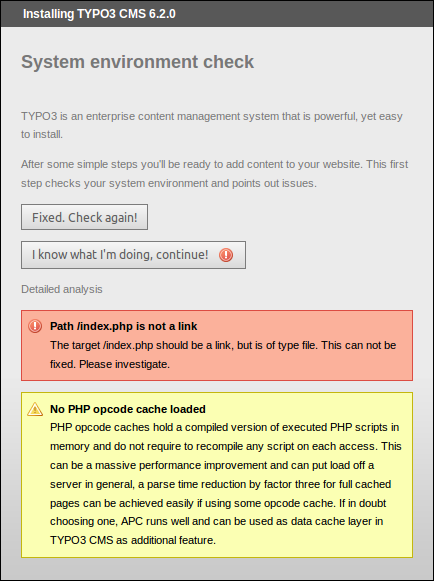
\includegraphics[width=0.8\linewidth]{Images/InstallTool/SystemEnvironmentCheck.png}
			\end{figure}
		\end{column}

	\end{columns}

\end{frame}

% ------------------------------------------------------------------------------
% Re-Development
% ------------------------------------------------------------------------------

\begin{frame}[fragile]
	\frametitle{Instalator (Install Tool)}
	\framesubtitle{Zmiany w instalatorze}

	\begin{columns}[T]

		\begin{column}{.5\textwidth}
			\begin{itemize}
				\item \underline{Drugi} krok pozwala użytkownikowi na konfiguracje połączenia do bazy danych
				\item Mozna wybrać sposób połączenia:
					\begin{itemize}
						\item przez port TCP/IP 
						\item połączenie przez gniazdo uniksowe
					\end{itemize}
				\item Inne systemy baz danych niż MySQL są również wspierane
			\end{itemize}
		\end{column}

		\begin{column}{.5\textwidth}
			\begin{figure}\vspace*{-0.4cm}
				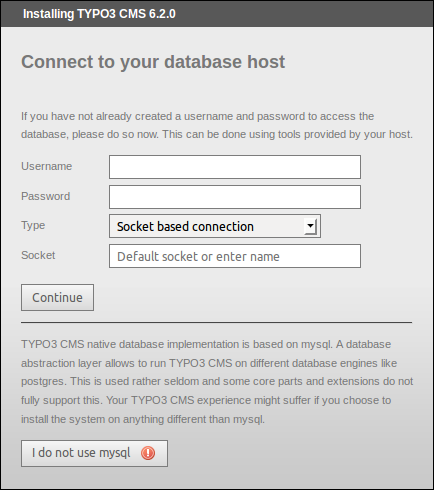
\includegraphics[width=0.8\linewidth]{Images/InstallTool/DatabaseConnectionDetails.png}
			\end{figure}
		\end{column}

	\end{columns}

\end{frame}

% ------------------------------------------------------------------------------
% Re-Development
% ------------------------------------------------------------------------------

\begin{frame}[fragile]
	\frametitle{Instalator (Install Tool)}
	\framesubtitle{Zmiany w instalatorze}

	\begin{columns}[T]

		\begin{column}{.5\textwidth}
			\begin{itemize}
				\item \underline{Trzeci} krok pozwala użytkownikom wybranie/utworzenie bazy danych (podobnie jak w TYPO3 < 6.2)
				\item \underline{Czwarty} krok pozwala na ustawienia hasła dla użytkownika "admin"\newline (to hasło staje się również hasłem do instalatora) oraz nazwy strony internetowej
			\end{itemize}
		\end{column}

		\begin{column}{.5\textwidth}
			\begin{figure}\vspace*{-0.4cm}
				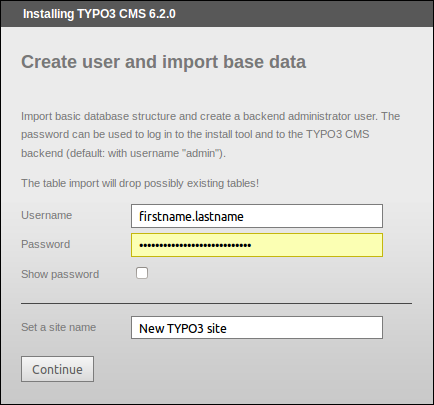
\includegraphics[width=0.8\linewidth]{Images/InstallTool/AdminPasswordAndSiteName.png}
			\end{figure}
		\end{column}

	\end{columns}

\end{frame}

% ------------------------------------------------------------------------------
% Clear All Cache
% ------------------------------------------------------------------------------

\begin{frame}[fragile]
	\frametitle{Instalator (Install Tool)}
	\framesubtitle{Czyszczenie całego cache'u ("Clear all cache")}

	\begin{itemize}
		\item Nowa funkcja "Clear all cache" w menu "Important actions" pozwala na wyczyszczenie całej pamięci podręcznej
		\item Działa nawet jeśli pamięć podręczna zawiera nieprawidłowy kod PHP
		\item Instalator jest dostępny pod adresem: \texttt{http://example.com/typo3/install} 
	\end{itemize}

	\begin{columns}[T]
		\begin{column}{.3\textwidth}
			\begin{figure}\vspace*{-0.4cm}
				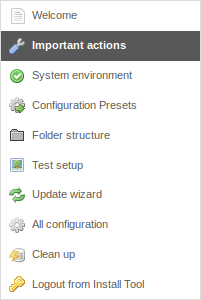
\includegraphics[width=0.7\linewidth]{Images/InstallTool/ImportantActions.png}
			\end{figure}
		\end{column}
		\begin{column}{.7\textwidth}
			\begin{figure}\vspace*{-0.4cm}
				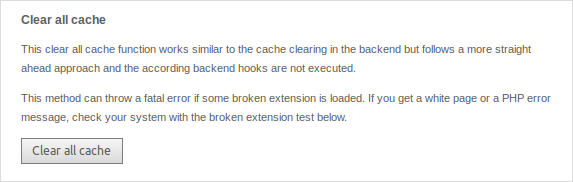
\includegraphics[width=0.9\linewidth]{Images/InstallTool/ClearAllCache.png}
			\end{figure}
		\end{column}
	\end{columns}

\end{frame}

% ------------------------------------------------------------------------------
% Clear All Cache
% ------------------------------------------------------------------------------

\begin{frame}[fragile]
	\frametitle{Instalator (Install Tool)}
	\framesubtitle{Czyszczenie całego cache'u ("Clear all cache")}

	Akcje wykonywane po wybraniu "Clear all cache":

	\begin{enumerate}
		\item Usuwana jest zawartość folderu \texttt{typo3temp/Cache}
		\item Czyszczone są tabele \texttt{cf\_*} w bazie danych
		\item Pliki \texttt{ext\_localconf.php} oraz \texttt{ext\_tables.php}\newline
			wczytywane są z rozszerzeń
		\item Uruchamiana jest metoda \texttt{flushCaches()} 
	\end{enumerate}

\end{frame}

% ------------------------------------------------------------------------------
% Check For Broken Extensions
% ------------------------------------------------------------------------------

\begin{frame}[fragile]
	\frametitle{Instalator (Install Tool)}
	\framesubtitle{Sprawdzenie niepewnych rozszerzeń (Check For Broken Extensions)}

	\begin{itemize}
		\item Nowa funkcja "Check For Broken Extensions" dostępna w menu "Important actions" pozwala sprawdzić,\newline
			czy zainstalowanie rozszerzenia nie popsuje instalacji
		\item Bardzo przydatna funkcja przy aktualizacji z TYPO3 4.5 do 6.2
	\end{itemize}

	\begin{columns}[T]
		\begin{column}{.3\textwidth}
			\begin{figure}\vspace*{-0.4cm}
				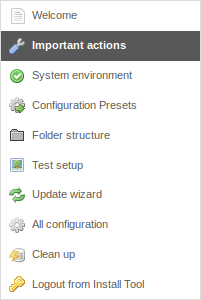
\includegraphics[width=0.7\linewidth]{Images/InstallTool/ImportantActions.png}
			\end{figure}
		\end{column}
		\begin{column}{.7\textwidth}
			\begin{figure}\vspace*{-0.4cm}
				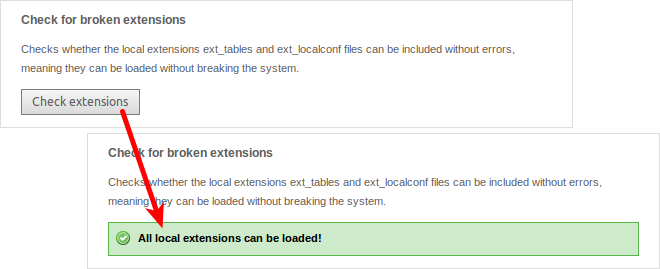
\includegraphics[width=1\linewidth]{Images/InstallTool/CheckForBrokenExtensions.png}
			\end{figure}
		\end{column}
	\end{columns}

\end{frame}

% ------------------------------------------------------------------------------
% Increased Security: Salted Passwords
% ------------------------------------------------------------------------------

\begin{frame}[fragile]
	\frametitle{Instalator (Install Tool)}
	\framesubtitle{Salted Passwords}

	\begin{itemize}
		\item Przy tworzeniu konta administracyjnego w Instalatorze,\newline
			hasło jest szyfrowane z użyciem ciągu zaburzającego (ang. salt)
			\smaller(wymaga rozszerzenia EXT:saltedpasswords)\normalsize
		\item Hasło do Instalatora jest również \textbf{solone} \newline
			\smaller(istniejące hasła są konwertowane automatycznie przy pierwszym logowaniu)\normalsize
	\end{itemize}

	\begin{columns}[T]
		\begin{column}{.3\textwidth}
			\begin{figure}\vspace*{-0.4cm}
				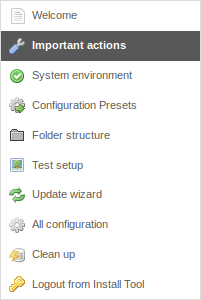
\includegraphics[width=0.7\linewidth]{Images/InstallTool/ImportantActions.png}
			\end{figure}
		\end{column}
		\begin{column}{.7\textwidth}
			\begin{figure}\vspace*{-0.4cm}
				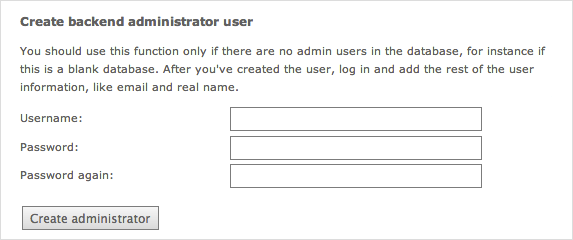
\includegraphics[width=0.9\linewidth]{Images/InstallTool/SaltedPasswords.png}
			\end{figure}
		\end{column}
	\end{columns}

\end{frame}

% ------------------------------------------------------------------------------
% Application Context
% ------------------------------------------------------------------------------

\begin{frame}[fragile]
	\frametitle{Instalator (Install Tool)}
	\framesubtitle{Kontekst Aplikacji (Application Context) (1)}

	\begin{itemize}
		\item TYPO3 >= 6.2 bierze pod uwagę \textbf{Kontekst Aplikacji}\newline
			\smaller(znany z TYPO3 Flow)\normalsize
		\item Zmienna środowiskowa \texttt{TYPO3\_CONTEXT} ustawia aktualny kontekst\newline
			\smaller(domyślnie: \texttt{Production}, pod-konteksty, np. \texttt{Production/Staging} są możliwe)\normalsize

			\begin{lstlisting}
				# File: .htaccess
				# Rules to set Application Context based on hostname:

				RewriteCond %{HTTP_HOST} ^dev\.example\.com$
				RewriteRule (.*) $1 [E=TYPO3_CONTEXT:Development]

				RewriteCond %{HTTP_HOST} ^www\.example\.com$
				RewriteRule (.*) $1 [E=TYPO3_CONTEXT:Production]

				# Sets an environment variable, which is then available to TYPO3 CMS:
				SetEnv TYPO3_CONTEXT Production
			\end{lstlisting}

	\end{itemize}

\end{frame}

% ------------------------------------------------------------------------------
% Presets of TYPO3_CONF_VAR Settings
% ------------------------------------------------------------------------------

\begin{frame}[fragile]
	\frametitle{Instalator (Install Tool)}
	\framesubtitle{Szablony ustawień TYPO3\_CONF\_VAR}

	\begin{columns}[T]
		\begin{column}{.5\textwidth}

			\begin{itemize}
				\item Niektóre ustawienia \texttt{TYPO3\_CONF\_VAR} mogą mieć rózną wartość w zależności od \textbf{Kontekstu Aplikacji}
				\item Wbudowane są 2 konteksty: "Production" oraz "Development"\newline
					(mozna tez tworzyć własne)
				\item Ustawienia takie jak "debug output", "deprecation log", "devIPmask" i inne takie jak logi systemu i poziomy logów
				
			\end{itemize}

		\end{column}
		\begin{column}{.5\textwidth}

			\begin{figure}\vspace*{-0.4cm}
				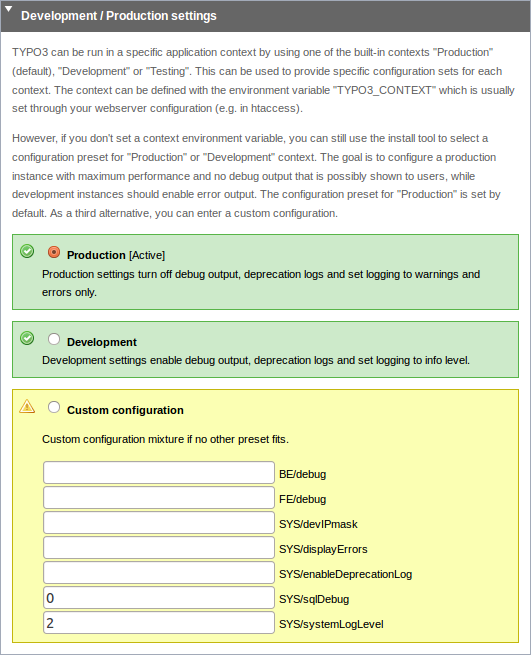
\includegraphics[width=0.8\linewidth]{Images/InstallTool/PresetsOfSettings.png}
			\end{figure}

		\end{column}
	\end{columns}

\end{frame}

% ------------------------------------------------------------------------------
% Improved Usability
% ------------------------------------------------------------------------------

\begin{frame}[fragile]
	\frametitle{Instalator (Install Tool)}
	\framesubtitle{Poprawiona Uzyteczność}

	\begin{columns}[T]
		\begin{column}{.5\textwidth}

			\begin{itemize}
				\item Poprawiona pozycja lewego \newline
					menu podczas skrolowania
					\begingroup\color{typo3red}\textbf{(1)}\endgroup
				\item Poprawiona pozycja przycisku "Write Configuration" na dole
					\begingroup\color{typo3red}\textbf{(2)}\endgroup
				\item Wpisy w "All Configuration" są pogrupowane (kliknij na nagłówek by rozwinąć sekcje) i posortowane
					\begingroup\color{typo3red}\textbf{(3)}\endgroup
			\end{itemize}

		\end{column}
		\begin{column}{.5\textwidth}

			\begin{figure}\vspace*{-0.4cm}
				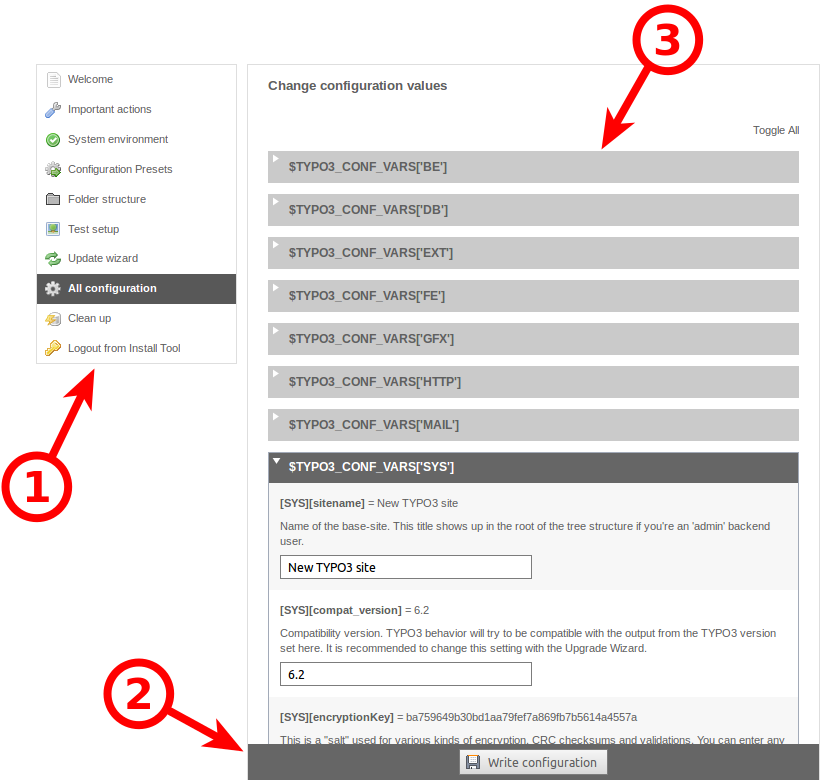
\includegraphics[width=0.8\linewidth]{Images/InstallTool/ImprovedUsability.png}
			\end{figure}

		\end{column}
	\end{columns}

\end{frame}

% ------------------------------------------------------------------------------
% Human-Friendly Error Codes
% ------------------------------------------------------------------------------

\begin{frame}[fragile]
	\frametitle{Instalator (Install Tool)}
	\framesubtitle{Bardziej przyjazne kody błędów}

	\begin{itemize}
		\item Znaczące słowa kluczowe mogą być uszyte dla poszczególnych opcji:\newline
			(TYPO3 < 6.2: tylko wartości numeryczne)
	\end{itemize}

	\begin{columns}[T]
		\begin{column}{.4\textwidth}
			\advance\leftskip+0.8cm

			\smaller
				\texttt{[SYS][errorHandlerErrors]}\newline
				\texttt{[SYS][exceptionalErrors]}\newline
				\texttt{[SYS][syslogErrorReporting]}\newline
				\texttt{[SYS][belogErrorReporting]}\newline
			\normalsize

		\end{column}
		\begin{column}{.6\textwidth}

			\begin{figure}\vspace*{-0.4cm}
				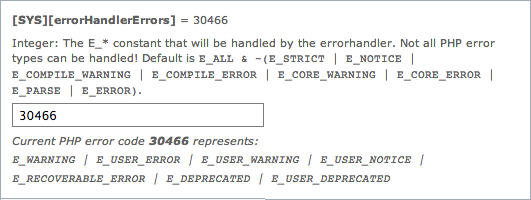
\includegraphics[width=0.9\linewidth]{Images/InstallTool/HumanFriendlyErrorCodes.png}
			\end{figure}

		\end{column}
	\end{columns}

	\vspace{0.2cm}

	\begin{itemize}
		\item Extbase ViewHelper \textbf{format.phpErrorCode} jest odpowiedzialny za konwersje wartości do kodów błędów PHP
	\end{itemize}

\end{frame}

% ------------------------------------------------------------------------------
% Errors In Folder Structure
% ------------------------------------------------------------------------------

\begin{frame}[fragile]
	\frametitle{Instalator (Install Tool)}
	\framesubtitle{Błędy w "Folder Structure"}

	\begin{itemize}
		\item Błędy w "Folder Structure" są podliczone i pokazane jako numer w kółku
	\end{itemize}

	\begin{figure}
		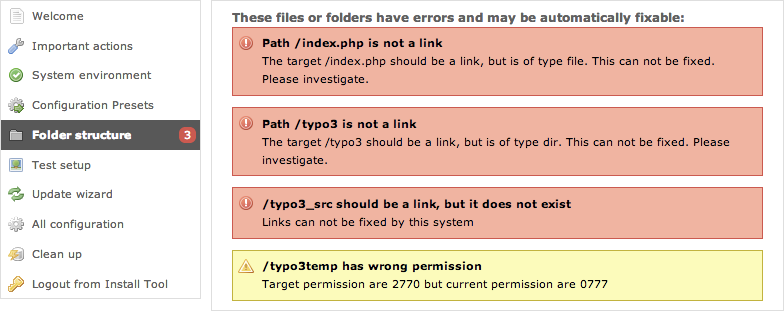
\includegraphics[width=0.95\linewidth]{Images/InstallTool/ErrorsInFolderStructure.png}
	\end{figure}

\end{frame}

% ------------------------------------------------------------------------------
% Core Updates
% ------------------------------------------------------------------------------

\begin{frame}[fragile]
	\frametitle{Instalator (Install Tool)}
	\framesubtitle{Aktualizacje}

	\begin{itemize}
		\item Aktualizacja TYPO3 do najnowszej wersji za pomocą kliknięcia w przycisk 
		\item Zmienna \texttt{TYPO3\_DISABLE\_CORE\_UPDATER=1} wyłącza tę funkcję
	\end{itemize}

	\begin{figure}
		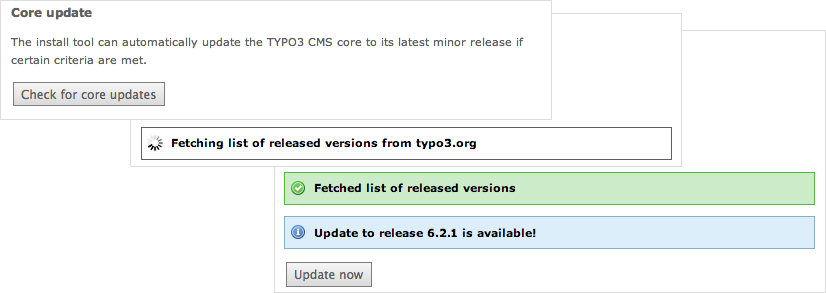
\includegraphics[width=0.95\linewidth]{Images/InstallTool/CoreUpdate.png}
	\end{figure}

\end{frame}

% ------------------------------------------------------------------------------
% Miscellaneous
% ------------------------------------------------------------------------------

\begin{frame}[fragile]
	\frametitle{Instalator (Install Tool)}
	\framesubtitle{Różne}

	\begin{itemize}
		\item Wszystkie formy są chronione przed atakiem CSRF(\textit{cross-site request forgery})
		\item Narzędzie instalacyjne używa uproszczonego "Fluid Standalone View"
		\item Załadowane są tylko podstawowe funkcje TYPO3\newline
			(wystąpienie błędu w \texttt{ ext\_localconf.php} lub \texttt{ext\_tables.php} nie może przerwać pracy instalatora)
		\item Nowy punkt startowy:	\tabto{3.2cm} \texttt{typo3/sysext/install/Start/Install.php}\newline
			Przedtem:				\tabto{3.2cm} \texttt{typo3/install/index.php}\newline
									\tabto{3.2cm} (istnieje przekierowanie ze starego do nowego\newline
									\tabto{3.2cm} URL)
	\end{itemize}

\end{frame}

% ------------------------------------------------------------------------------
% Miscellaneous
% ------------------------------------------------------------------------------

\begin{frame}[fragile]
	\frametitle{Instalator (Install Tool)}
	\framesubtitle{Różne}

	\begin{itemize}
		\item Po wyłączeniu pamięci podręcznej możliwe jest używanie instalatora nawet jeśli zawierał on nieprawidłowy kod PHP
		\item Sprawdź czy opcja PHP \texttt{xdebug.max\_nesting\_level} pokazuje wartość 250 lub wyższą (domyślna wartość "100" prawdopodobnie może powodować problemy)
		\item "Relaxed permission check":

			\small
				Jeśli główny folder nie posiada poprawnie ustawionych praw (np "2770"), 
				a te prawa nie mogą zostać ustawione np. dlatego ze folder instalacji nie 
				należy do użytkownika który uruchomił instalator, pierwszy krok instalacji
				zostanie przerwany.
				Opcja "targetPermissionRelaxed" zmniejsza zapotrzebowanie na prawa jeśli nie są 
				idealne i pozwala na kontynuowanie instalacji do momentu do którego będzie możliwe
				tworzenie podfolderów.
			\normalsize

	\end{itemize}

\end{frame}

% ------------------------------------------------------------------------------
% Miscellaneous
% ------------------------------------------------------------------------------

\begin{frame}[fragile]
	\frametitle{Instalator (Install Tool)}
	\framesubtitle{Różne}

	\begin{itemize}
		\item Usunięto opcje (keys) z Instalatora\newline
			\small(i następnie z pliku \texttt{LocalConfiguration.php}, oraz:\normalsize
	\end{itemize}

	\begin{columns}[T]
		\begin{column}{.5\textwidth}
			\advance\leftskip+0.8cm
			\smaller
				\texttt{BE/loginLabels}\newline
				\texttt{BE/loginNews}\newline
				\texttt{BE/useOnContextMenuHandler}\newline
				\texttt{EXT/em\_mirrorListURL}\newline
				\texttt{EXT/em\_wsdlURL}\newline
				\texttt{EXT/extList}\newline
				\texttt{EXT/extList\_FE}\newline
				\texttt{EXT/noEdit}\newline
			\normalsize
		\end{column}
		\begin{column}{.5\textwidth}
			\smaller
				\texttt{FE/defaultTypoScript\_editorcfg}\newline
				\texttt{FE/simulateStaticDocuments}\newline
				\texttt{GFX/noIconProc}\newline
				\texttt{GFX/TTFLocaleConv}\newline
				\texttt{SYS/additionalAllowedClassPrefixes}\newline
				\texttt{SYS/caching/cacheBackends}\newline
				\texttt{SYS/caching/cacheFrontends}\newline
				\texttt{SYS/extCache}\newline
				\texttt{SYS/T3instID}\newline
			\normalsize
		\end{column}

	\end{columns}

\end{frame}

% ------------------------------------------------------------------------------

